\documentclass[12pt, a4paper]{book}

\usepackage{fancyhdr}
\usepackage[left=4cm, right=4cm, top=4cm, bottom=4cm]{geometry}
\usepackage[utf8]{inputenc}
\usepackage[table]{xcolor}
\usepackage[hidelinks]{hyperref}
\usepackage{amsmath}
\usepackage{enumitem}
\usepackage{graphicx}
\usepackage{amsfonts}
\usepackage{booktabs}
\usepackage{subcaption}
\usepackage[justification=centering]{caption}
\usepackage{xepersian}

\DeclareMathOperator*{\argmax}{argmax}
\DeclareMathOperator*{\argmin}{argmin}
\newcolumntype{L}{>{$}l<{$}} % math-mode version of "l" column type

\newcommand{\coursetitle}{شبکه‌های عصبی}
\newcommand{\doctitle}{تمرین هشتم}
\newcommand{\name}{محمدرضا غفرانی}
\newcommand{\studentno}{400131076}
\newcommand{\todaydate}{\today}

\settextfont{Sahel}
\setlatintextfont{EB Garamond}

\pagestyle{fancy}
\lhead{\textbf{\doctitle}}
\chead{\name}
\rhead{\todaydate}

\begin{document}

\begin{flushleft}
    \name \\
    \studentno \\
    \todaydate
\end{flushleft}

\begin{center}
    \huge
    \textbf{\coursetitle}
    \break
    \large
    \doctitle
\end{center}

% suppress the fancy header on the first page only
\thispagestyle{plain}

\section*{سوال یک}

برای تبدیل جملات به توکن‌ها از مدلی که برای این مجموعه داده
بهینه شده است\LTRfootnote{\href{https://www.tensorflow.org/text/guide/subwords_tokenizer}{\lr{https://www.tensorflow.org/text/guide/subwords\_tokenizer}}}
استفاده می‌کنیم. این توکن‌کننده علاوه بر تبدیل جملات به توکن‌ها پیش‌پردازش‌های دیگری نظیر
یکسان‌سازی\LTRfootnote{Normalize} متون و کوچک‌کردن\LTRfootnote{lowercase} تمامی کلمات
را انجام می‌دهد. پیش‌پردازش دیگری که ما انجام می‌دهیم حذف جملاتی که طول آن‌ها بسیار زیاد است.
هدف از حذف این جملات بهتر‌کردن عملکرد مدل با حذف این داده‌های پرت است.

برای حذف کلماتی که اندازه آن‌ها از یک حد آستانه‌ای بیشتر است، ابتدا نیاز است تا درکی از طول جملات
موجود در مجموعه داده داشته باشیم. بنابراین طول تمامی جملات را در مجموعه داده استخراج و در شکل
\ref{sentence_lengths} رسم می‌کنیم. بنابراین این شکل طول جملات معمولا تا ۱۰۰ کلمه است این حالی که
در همین مجموعه داده جمله‌ای با طول ۳۹۱ کلمه نیز وجود دارد.
بنابراین توضیحات ۱۲۸ طول معقولی برای حداکثر جمله به نظر می‌رسد.

\begin{figure}[h]
    \centering
    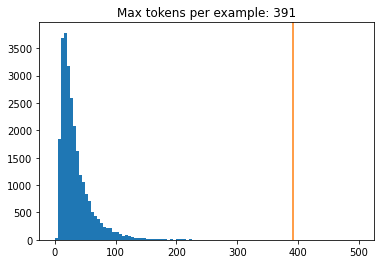
\includegraphics[width=0.4\linewidth]{images/lengths.png}
    \caption{طول جملات موجود در مجموعه داده}
    \label{sentence_lengths}
\end{figure}

\section*{سوال دوم}

در شکل \ref{position_encoding} تعبیه مکانی که برای هر کلمه در نظر گرفته می‌شود آورده شده است.
این تعبیه مکانی برای جمله‌ای در اندازه ۲۰۴۸ کلمه قابل استفاده است. ما در این جا با توجه
به این که طول جملات ورودی بسیار کوچک‌تری داریم (طول جملات ورودی و خروجی برابر حداکثر ۱۲۸ در نظر گرفته شده‌اند)
بنابراین نیازی به استفاده از همه این تعبیه نداشته و از بخش بسیار کوچک آن برای ساخت تعبیه مکانی کلمه استفاده می‌کنیم.

\begin{figure}
    \centering
    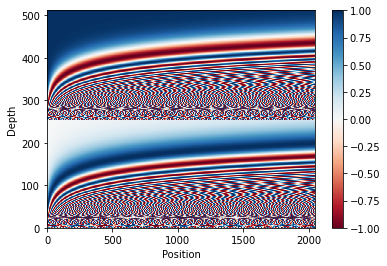
\includegraphics[width=0.5\linewidth]{images/position.png}
    \caption{تعبیه مکانی برای هر کلمه در جمله‌ای به طول ۲۰۴۸}
    \label{position_encoding}
\end{figure}

\section*{سوال سوم}

\subsection*{قسمت الف}

در مقاله‌ \lr{Attension is all you need!} پیشنهاد شده است که از بهینه‌ساز \lr{Adam} با نرخ یادگیری که
مقدار آن از طریق فرمول \ref{lrate_formula} محاسبه می‌شود استفاده شود. به همین دلیل ما نیز از همین تابع خطا برای یادگیری
استفاده می‌کنیم.

\begin{eqnarray}
    \eta = d_{model}^{-0.5} * \min(\text{\lr{step\_num}}^{-0.5}, \text{\lr{step\_num}} \cdot \text{\lr{warmup\_step}}^{-1.5})
    \label{lrate_formula}
\end{eqnarray}

در شکل \ref{lrate_figure} تغییرات نرخ یادگیری پیشنهاد شده در فرمول بالا در گام‌های یادگیری دیده می‌شود. در ابتدا نمودار صعودی
بوده و مقدار نرخ یادگیری بیشتر و بیشتر می‌شود. با رسیدن به نقطه بیشینه که محل تلاقی خط $\frac{\text{\lr{step\_num}}}{\text{\lr{warmup\_step}}^{1.5}}$
و منحنی $\frac{1}{\text{\lr{step\_num}}^{-0.5}}$ است؛ شیب نمودار رو به پایین شده و مقدار نرخ یادگیری و در نتیجه
آزادی عمل مدل رفته‌رفته کم‌وکم‌تر می‌شود.

\begin{figure}[h]
    \centering
    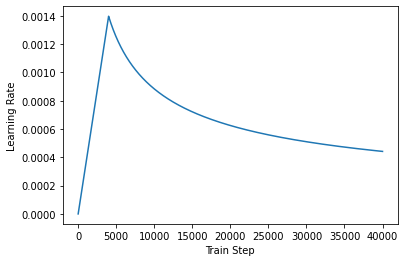
\includegraphics[width=0.5\linewidth]{images/lrate_fig.png}
    \caption{تغییرات نرخ یادگیری بر اساس فرمول \ref{lrate_formula}}
    \label{lrate_figure}
\end{figure}

\subsection*{قسمت ب}

در شکل \ref{attention} نحوه توجه مدل به ورودی‌ها برای تولید خروجی مشاهده می‌شود.
در \lr{Head1} و \lr{Head4} مدل از یک دید کلی برای به دست آوردن تعبیه هر کلمه بر اساس متن بهره می‌گیرد.

در \lr{Head3} با توجه به آن که بیشتر توجه مدل روی دو کلمه \lr{light} با کلمه متناظرش و کلمه \lr{is} با
ترجمه متناظرش است بنابراین هدف مدل از این توجه تطبیق دادن اسم و فعل است.

در \lr{Head2}، \lr{Head5}، \lr{Head6} و \lr{Head7} بیشتر توجه مدل روی گروه‌های اسمی و فعلی و به خصوص
هسته این گروه‌هاست. مثلا در \lr{Head2} مدل توجه زیادی به کلمه‌های \lr{desparece} و ترجمه معادل آن
یعنی \lr{is never gone} کرده است. بعلاوه در همان \lr{Head2} مدل توجه زیادی به انتهای جمله داشته و
به نظر می‌رسد که نمی‌خواسته طول ترجمه‌ای که ارائه می‌دهد از یک اندازه‌ای بیشتر باشد. در \lr{Head5} و \lr{Head6} مدل علاوه بر
گروه‌های اصلی نظیر اسمی و فعلی به گروه قیدی \lr{nunca} نیز توجه کرده و این مورد را در ترجمه دخیل کرده است.

\begin{figure}[h]
    \centering
    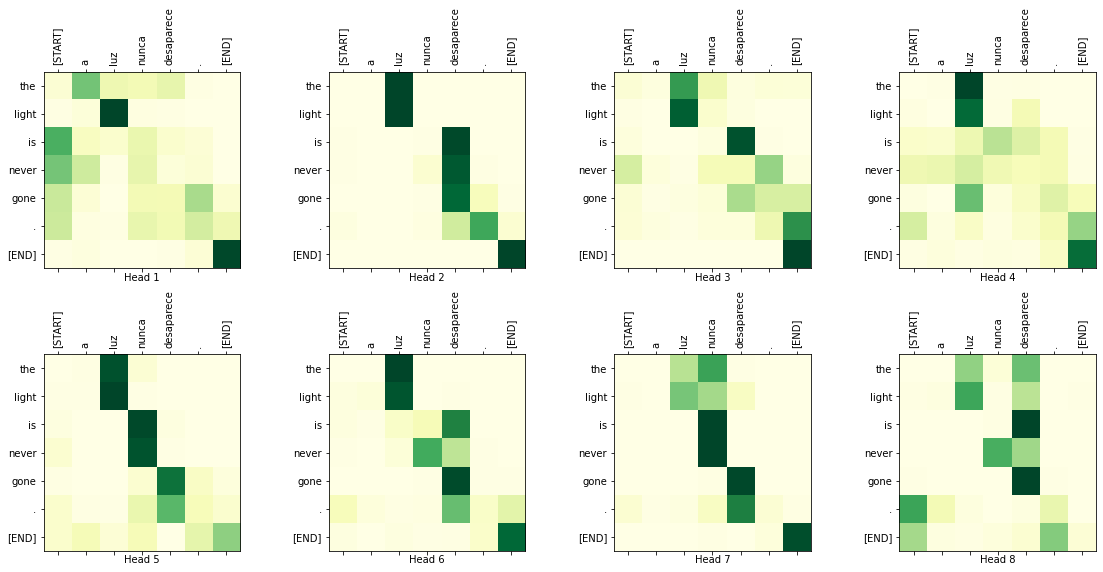
\includegraphics[width=\linewidth]{images/attention.png}
    \caption{نقشه توجه مدل به ورودی‌ها}
    \label{attention}
\end{figure}

\subsection*{قسمت ج}

در ادامه عملکرد مدل بر روی ۲۰ تا از جملات موجود در داده آزمون مشاهده می‌شود. با توجه به موارد پایین عملکرد مدل قابل
است و اکثر ترجمه قابل قبول را ارائه داده است برای مثال ۱۴ مدل بر اساس ورودی که جمله خبری است خروجی را تولید کرده
است؛ در حالی که ترجمه انسانی بر حسب مفهوم و سلیقه ترجمه را به شکل جمله پرسشی انجام داده است.
بعلاوه در بعضی موارد ترجمه خروجی دقیقا جمله مرجع است. مثال ۵ یکی از این موارد است. دقت داشته باشید که
از آن‌ جا که این آزمون روی داده‌ تست انجام شده است بنابراین یکسان بودن خروجی مدل و جمله مرجع بسیار
حائز اهمیت است. بعضا ایراد‌هایی نیز در عملکرد مدل مشاهده می‌شود.
برای مثال در مثال شماره ۱۳ مدل نتوانسته است به خوبی
قسمت \lr{how much negative energy it takes} را ترجمه کند.
یا مثلا در مثال شماره ۱۰ مدل کلمه \lr{now} را دوبار در خروجی تکرار کرده است.

\begin{figure}
    \begin{subfigure}{\linewidth}
        \begin{flushright}
        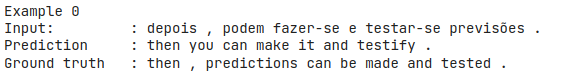
\includegraphics[width=\linewidth]{images/examples/1.png}
        \end{flushright}
    \end{subfigure}
    \break
    \begin{subfigure}{\linewidth}
        \begin{flushright}
        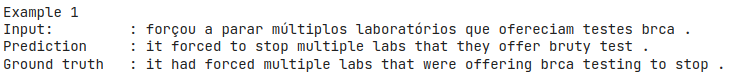
\includegraphics[width=\linewidth]{images/examples/2.png}
        \end{flushright}
    \end{subfigure}
    \break
    \begin{subfigure}{\linewidth}
        \begin{flushright}
        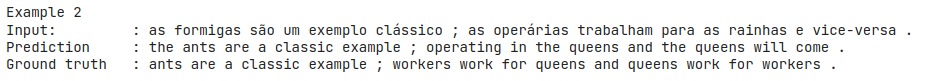
\includegraphics[width=\linewidth]{images/examples/3.png}
        \end{flushright}
    \end{subfigure}
    \break
    \begin{subfigure}{\linewidth}
        \begin{flushright}
        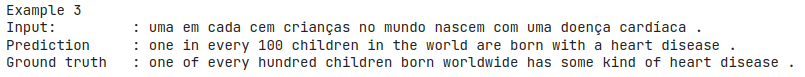
\includegraphics[width=\linewidth]{images/examples/4.png}
        \end{flushright}
    \end{subfigure}
    \break
    \begin{subfigure}{\linewidth}
        \begin{flushright}
        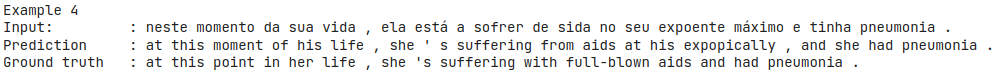
\includegraphics[width=\linewidth]{images/examples/5.png}
        \end{flushright}
    \end{subfigure}
    \break
    \begin{subfigure}{\linewidth}
        \begin{flushright}
        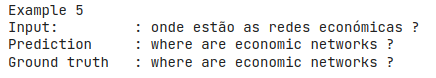
\includegraphics[width=\linewidth]{images/examples/6.png}
        \end{flushright}
    \end{subfigure}
    \break
    \begin{subfigure}{\linewidth}
        \begin{flushright}
        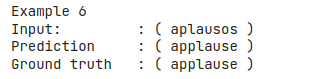
\includegraphics[width=\linewidth]{images/examples/7.png}
        \end{flushright}
    \end{subfigure}
    \break
    \begin{subfigure}{\linewidth}
        \begin{flushright}
        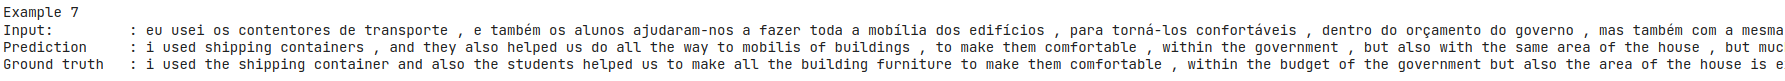
\includegraphics[width=\linewidth]{images/examples/8.png}
        \end{flushright}
    \end{subfigure}
    \break
\end{figure}
\begin{figure}[h]
    \ContinuedFloat
    \begin{subfigure}{\linewidth}
        \begin{flushright}
        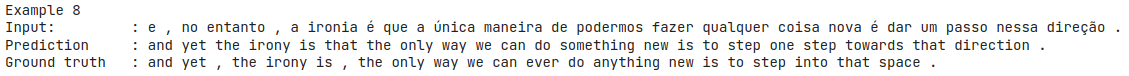
\includegraphics[width=\linewidth]{images/examples/9.png}
        \end{flushright}
    \end{subfigure}
    \break
    \begin{subfigure}{\linewidth}
        \begin{flushright}
        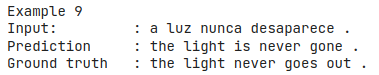
\includegraphics[width=\linewidth]{images/examples/10.png}
        \end{flushright}
    \end{subfigure}
    \break
    \begin{subfigure}{\linewidth}
        \begin{flushright}
        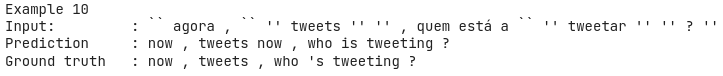
\includegraphics[width=\linewidth]{images/examples/11.png}
        \end{flushright}
    \end{subfigure}
    \break
    \begin{subfigure}{\linewidth}
        \begin{flushright}
        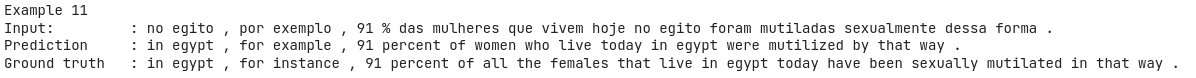
\includegraphics[width=\linewidth]{images/examples/12.png}
        \end{flushright}
    \end{subfigure}
    \break
    \begin{subfigure}{\linewidth}
        \begin{flushright}
        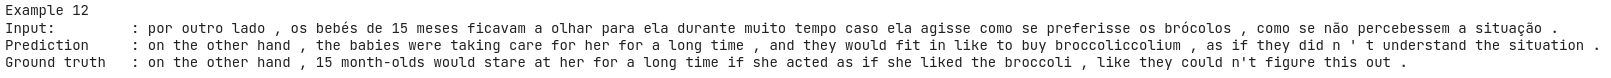
\includegraphics[width=\linewidth]{images/examples/13.png}
        \end{flushright}
    \end{subfigure}
    \break
    \begin{subfigure}{\linewidth}
        \begin{flushright}
        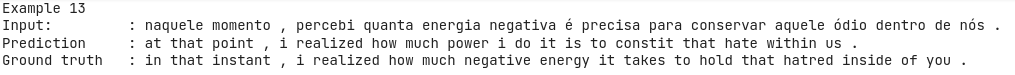
\includegraphics[width=\linewidth]{images/examples/14.png}
        \end{flushright}
    \end{subfigure}
    \break
    \begin{subfigure}{\linewidth}
        \begin{flushright}
        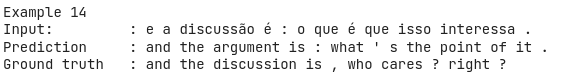
\includegraphics[width=\linewidth]{images/examples/15.png}
        \end{flushright}
    \end{subfigure}
    \break
    \begin{subfigure}{\linewidth}
        \begin{flushright}
        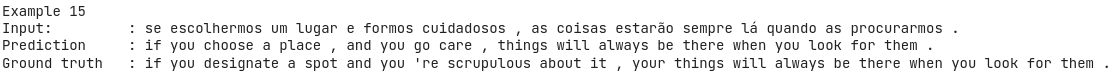
\includegraphics[width=\linewidth]{images/examples/16.png}
        \end{flushright}
    \end{subfigure}
    \break
    \begin{subfigure}{\linewidth}
        \begin{flushright}
        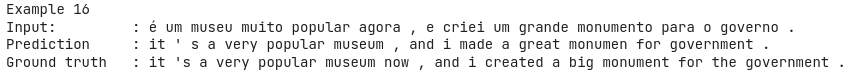
\includegraphics[width=\linewidth]{images/examples/17.png}
        \end{flushright}
    \end{subfigure}
    \break
    \begin{subfigure}{\linewidth}
        \begin{flushright}
        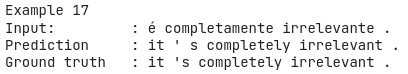
\includegraphics[width=\linewidth]{images/examples/18.png}
        \end{flushright}
    \end{subfigure}
    \break
    \begin{subfigure}{\linewidth}
        \begin{flushright}
        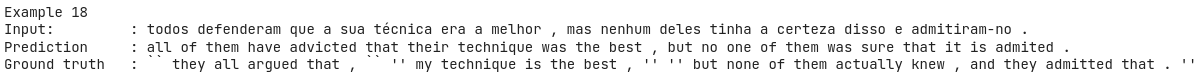
\includegraphics[width=\linewidth]{images/examples/19.png}
        \end{flushright}
    \end{subfigure}
    \break
    \begin{subfigure}{\linewidth}
        \begin{flushright}
        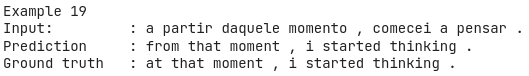
\includegraphics[width=\linewidth]{images/examples/20.png}
        \end{flushright}
    \end{subfigure}
    \break
\end{figure}



\end{document}